\section{Theoretische Grundlage}
\label{sec:Theorie}
Zur Beugung von Licht kommt es, wenn die Abmessung des Hinderniss in der Größenordung der Wellenlänge $\lambda$ liegt. Dabei kommt es zur Abweichung des Lichtes von der Geometrischen Optik. Für den Versuch wird angenommen das der Schirm eine weite Entfernung zur  Blende aufweist, so dass die Frauenhofer-Näherung genutzt werden kann. In Abbildung \ref{fig:Fra} ist zu sehen das das Licht jeweils um den Winkel $\phi$ gebeugt wird.
\begin{figure}
  \centering
  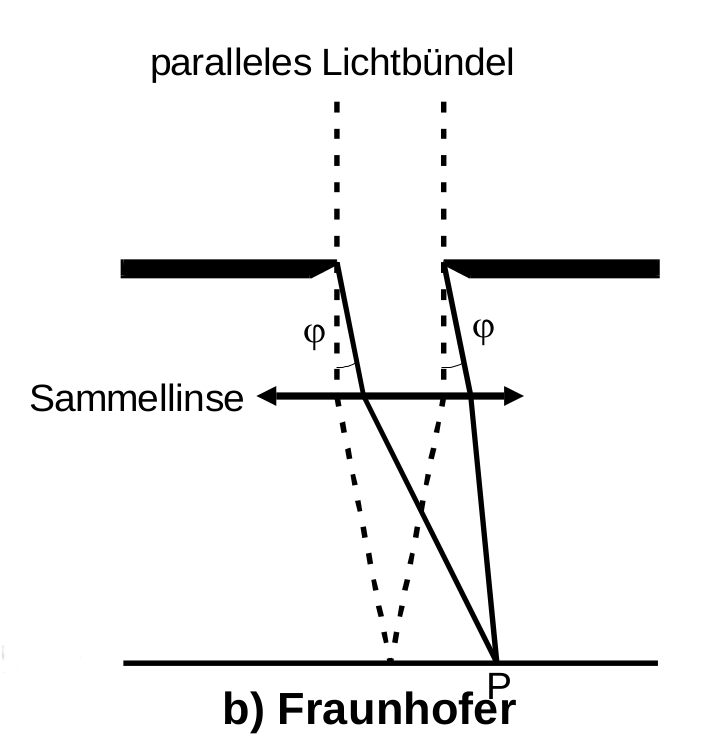
\includegraphics[height=6cm]{picture/Frauenhofer.png}
  \caption{Frauenhofer Beugung}
  \label{fig:Fra}
\end{figure}
Anhand des Huygensschen Prinzip lässt sich bei hinreichend großer Intensität die Interferenzbeschreibung beschreiben. Es besagt einerseits, dass jeder Punkt einer Wellenfront Ausgangspunkt einer neuen Kugelwelle ist, als auch dass die Einhüllende der Elementarwellen die neue Wellenfront ergibt. Um eine Aussage in einenm Punkt zu machen, müssen aufgrund des Huygensschen Prinzip alle Wellen die in diesem Punkt ankommen überlagtert werden. Der einfacherheit halber wird zunächst ein Einzelspalt betrachtet und anschließend auf andere Querschnitte geschlossen. Beim Einzelspalt müssen dafür die einzelnen Amplituden eines Strahlenbündel  unter dem entsprechenden Ablenkungswinkel $\phi$ summiert werden.
\begin{figure}
  \centering
  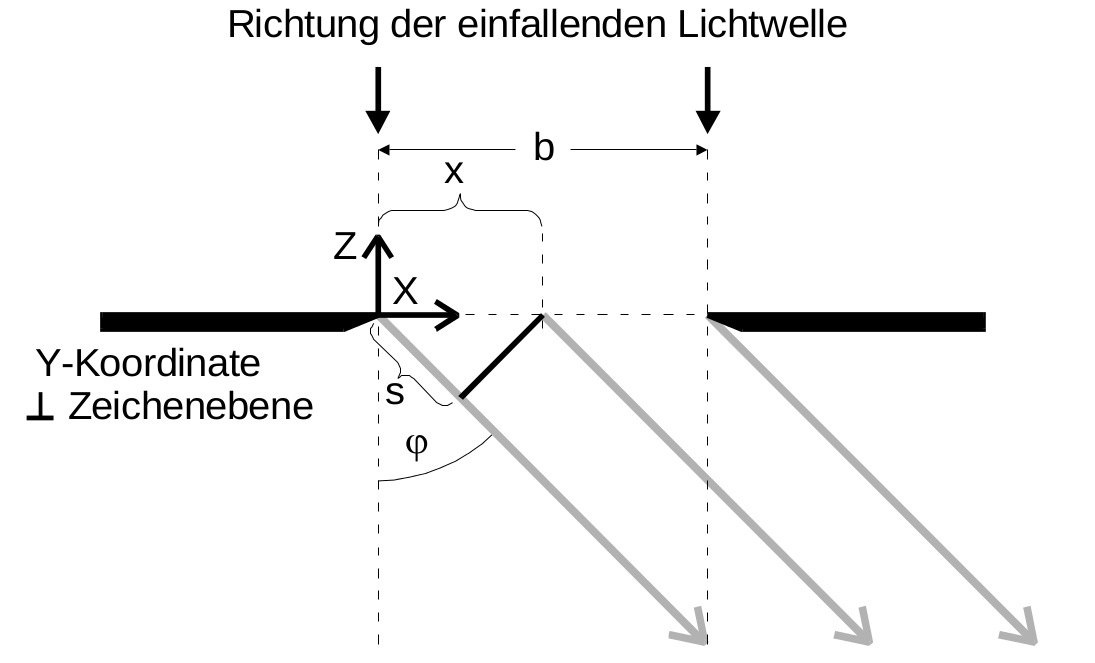
\includegraphics[height=5cm]{picture/doppelspalt.png}
  \caption{Phasenbeziehung zwischen zwei Teilstrahlen}
  \label{fig:dop}
\end{figure}
Es wird eine ebene Welle mit der Feldstärke
\begin{equation}
  A(z,t)= A_0 \textbf{exp} \left( i \left( \omega t - \frac{2 \pi z}{\lambda}   \right) \right)
  \label{eqn:welle}
\end{equation}
angenommen die durch den Spalt mit Breite $b$ einfällt. Der Phasenunteschied zweier Strahlen mit dem Abstand $x$ beträgt:
\begin{equation}
  \delta = \frac{2 \pi x sin(\phi)}{\lambda}
  \label{eqn:phase}
\end{equation}
Durch Integration über alle Strahlen die um den Winkel $\phi$ abgelengt sind ergibt sich:
\begin{equation}
  B(z,t,\phi) = A_0 \textbf{exp} \left( i \left( \omega t - \frac{2 \pi z}{\lambda} \right) \right) \cdot \textbf{exp} \left( \frac{\pi b sin(\phi)}{\lambda} \right)
  \label{}
\end{equation}
Für die experimentelle Auswertung müssen die Exponentialfunktionen nicht weiter betrachtet werden, da diese ausschließlich Informationen über die Phase der Funktion enthalten. Da aufgrund der hohen Lichtfrequenz eine Messung der Amplitude nicht möglich ist muss die Intensitätsverteilung  ermittelt werden.
\begin{equation}
  I(\phi) \propto B(\phi)^2 = A_0^2 b^2 \left( \frac{\lambda}{\pi b sin \phi} \right)^2 sin^2 \left( \frac{\pi b sin \phi}{\lambda} \right)
  \label{eqn:I}
\end{equation}
Die Intensitätsverteilung des $I(\phi)$ des Doppelspalts beruht darauf das im Abstand $s$ ein zweiter Einzelspalt der Breite $b$ überlagert wird.
\begin{equation}
  I(\phi) \propto B(\phi)^2 = 4cos^2\left( \frac{\pi s sin(\phi)}{\lambda} \right) \left( \frac{\lambda}{\pi b sin \phi} \right)^2 sin^2 \left( \frac{\pi b sin \phi}{\lambda} \right)
  \label{eqn:Id}
\end{equation}

\subsection{Fehlerrechnung}
Sämtliche Fehlerrechnungen werden mit Hilfe von Python 3.4.3 durchgeführt.
\subsubsection{Mittelwert}
Der Mittelwert einer Messreihe $x_\text{1}, ... ,x_\text{n}$ lässt sich durch die Formel
\begin{equation}
	\overline{x} = \frac{1}{N} \sum_{\text{k}=1}^\text{N} x_k
	\label{eqn:ave}
\end{equation}
berechnen. Die Standardabweichung des Mittelwertes beträgt
\begin{equation}
	\Delta \overline{x} = \sqrt{ \frac{1}{N(N-1)} \sum_{\text{k}=1}^\text{N} (x_\text{k} - \overline{x})^2}
	\label{eqn:std}
\end{equation}

\subsubsection{Gauß'sche Fehlerfortpflanzung}
Wenn $x_\text{1}, ..., x_\text{n}$ fehlerbehaftete Messgrößen im weiteren Verlauf benutzt werden, wird der neue Fehler $\Delta f$ mit Hilfe der Gaußschen Fehlerfortpflanzung angegeben.
\begin{equation}
	\Delta f = \sqrt{\sum_{\text{k}=1}^\text{N} \left( \frac{ \partial f}{\partial x_\text{k}} \right) ^2 \cdot (\Delta x_\text{k})^2}
	\label{eqn:var}
\end{equation}

\subsubsection{Lineare Regression}
Die Steigung und y-Achsenabschnitt einer Ausgleichsgeraden werden gegebenfalls mittels Linearen Regression berechnet.
\begin{equation}
	y = m \cdot x + b
	\label{eqn:reg}
\end{equation}
\begin{equation}
	m = \frac{ \overline{xy} - \overline{x} \overline{y} } {\overline{x^2} - \overline{x}^2}
	\label{eqn:reg_m}
\end{equation}
\begin{equation}
	b = \frac{ \overline{x^2}\overline{y} - \overline{x} \, \overline{xy}} { \overline{x^2} - \overline{x}^2}
	\label{eqn:reg_b}
\end{equation}
